% Section 2: model problem, the computational task, and the two kinds of
% representation singularity. Cell notation follows draft/bie-siam Section 2.1.
\section{Model problem and computational task}\label{sec:model}

\subsection{Periodic media with a line defect}\label{sec:geometry}
For $s\in\{-,+\}$ let $\rho_s$ be a coefficient with periods $L_s>0$ in $x$ and
$d>0$ in $y$. The two sides share the period $d$; $L_-$ and $L_+$ may differ.
Each $\rho_s$ is piecewise constant. In a common background value
$\rho_{\mathrm e}>0$, every period cell of $\rho_s$ contains finitely many
simply connected rods with $C^2$ boundaries and constant values. The
coefficient $\rho$ of the waveguide equals $\rho_-$ for $x<x_-$ and $\rho_+$
for $x>x_+$. The \emph{defect cell} $(x_-,x_+)\times I_d$, with $x_\pm=\pm L_0/2$ and
$I_d:=(-d/2,d/2)$, contains one further rod $\Omega_0$ or none. All rod
closures stay away from the cell boundaries. We write
$0<\rin\le\rho\le\rax$ and $B:=\RR\times I_d$. The two \emph{periodic
half-strips} are $S_-=(-\infty,x_-)\times I_d$ and $S_+=(x_+,\infty)\times I_d$, with
coefficients $\rho_-$ and $\rho_+$; \cref{fig:model-geometry} shows the geometry.

The defect cell and the $j$th periodicity cells of $S_+$ and $S_-$ ($j\ge0$) are
\[
\begin{gathered}
  \mathcal C_0=(x_-,x_+)\times I_d,\qquad
  \mathcal C_{j,+}=(x_++jL_+,\,x_++(j+1)L_+)\times I_d,\\
  \mathcal C_{j,-}=(x_--(j+1)L_-,\,x_--jL_-)\times I_d .
\end{gathered}
\]
The vertical lines $\{x_\pm\}\times I_d$ are the \emph{artificial (vertical)
boundaries} of the defect cell; the lines between consecutive periodicity
cells are
the \emph{walls}. Every artificial boundary and every wall lies in a vertical
strip of pure background between two groups of rods. We call the largest such
open strip containing a given line its \emph{gap strip}, and its width $w$ the
gap width; $w_{\min}$ denotes the smallest gap width over all artificial
boundaries and walls. The position of these lines inside their gap strips is
a free parameter of the computation. When we speak of \emph{moving an
artificial boundary}, we mean moving this line inside its gap strip, which
changes no physical quantity.

% Geometry of the two periodic half-strips and the line defect in Section 2.1.
\begin{figure}[htbp]
\centering
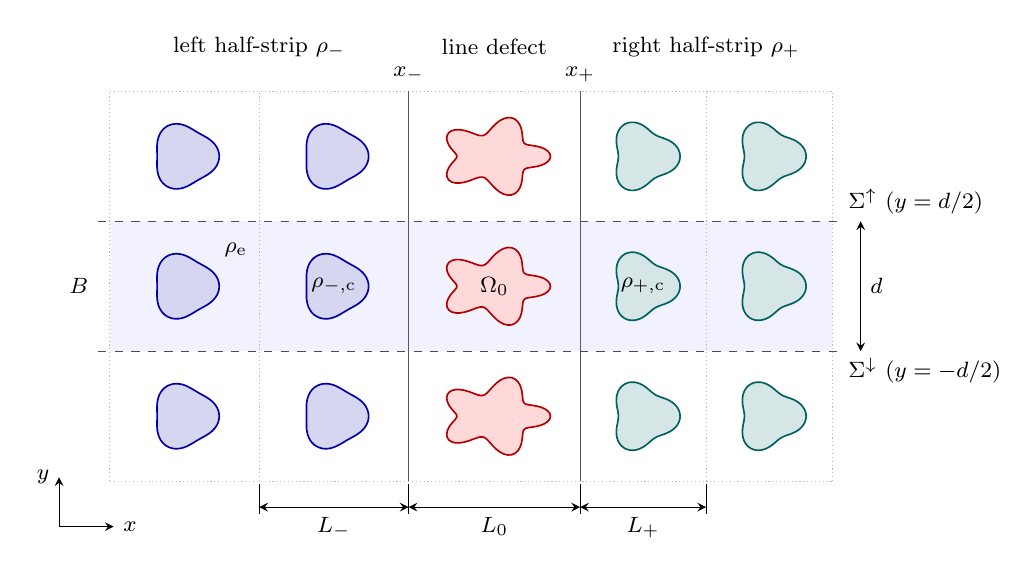
\begin{tikzpicture}[x=1.65cm,y=1.65cm,font=\footnotesize,>=stealth,
  cell wall/.style={gray!55,densely dotted,thin},
  seam/.style={black!70,dashed,thin},
  measure/.style={<->,thin},
  pics/lead rod/.style args={#1/#2}{code={
    \filldraw[draw=#1,fill=#1!16,line width=.6pt]
      plot[domain=0:360,samples=73,variable=\t]
      ({.24*(1+#2*cos(3*\t))*cos(\t)/sqrt(1+#2*#2/2)},
       {.24*(1+#2*cos(3*\t))*sin(\t)/sqrt(1+#2*#2/2)}) -- cycle;}},
  pics/defect rod/.style={code={
    \filldraw[draw=red!70!black,fill=red!15,line width=.6pt]
      plot[domain=0:360,samples=91,variable=\t]
      ({.24*(1.5+.3*cos(5*\t))*cos(\t)},
       {.24*(1+.3*cos(5*\t))*sin(\t)}) -- cycle;}}]
  % Two full periodicity cells on each side; three transverse periods.
  \fill[blue!5] (-2.96,-.5) rectangle (2.60,.5);
  \foreach \x in {-2.96,-1.81,1.63,2.60}
    \draw[cell wall] (\x,-1.5) -- (\x,1.5);
  \foreach \y in {-1.5,1.5}
    \draw[cell wall] (-2.96,\y) -- (2.60,\y);
  \foreach \x in {-.66,.66}
    \draw[black!65,thin] (\x,-1.5) -- (\x,1.5);
  \foreach \y in {-.5,.5}
    \draw[seam] (-3.05,\y) -- (2.69,\y);
  \foreach \y in {-1,0,1} {
    \foreach \x in {-2.385,-1.235}
      \pic at (\x,\y) {lead rod={blue!65!black/.12}};
    \pic at (0,\y) {defect rod};
    \foreach \x in {1.145,2.115}
      \pic at (\x,\y) {lead rod={teal!75!black/.20}};
  }
  \node at (-1.81,1.84) {left half-strip $\rho_-$};
  \node at (0,1.84) {line defect};
  \node at (1.63,1.84) {right half-strip $\rho_+$};
  \node[above] at (-.66,1.5) {$x_-$};
  \node[above] at (.66,1.5) {$x_+$};
  \node at (0,0) {$\Omega_0$};
  \node at (-1.99,.28) {$\rho_{\mathrm e}$};
  \node at (-1.235,0) {$\rho_{-,\mathrm c}$};
  \node at (1.145,0) {$\rho_{+,\mathrm c}$};
  \node[left] at (-3.05,0) {$B$};
  \draw[measure] (2.82,-.5) -- node[right] {$d$} (2.82,.5);
  \node[above right,inner sep=1pt] at (2.70,.53)
    {$\Sigma^\uparrow\ (y=d/2)$};
  \node[below right,inner sep=1pt] at (2.70,-.53)
    {$\Sigma^\downarrow\ (y=-d/2)$};
  \foreach \a/\b/\period in {-1.81/-.66/L_-,-.66/.66/L_0,.66/1.63/L_+} {
    \draw[thin] (\a,-1.52) -- (\a,-1.75);
    \draw[measure] (\a,-1.70) -- node[below] {$\period$} (\b,-1.70);
  }
  \draw[thin] (1.63,-1.52) -- (1.63,-1.75);
  \draw[->] (-3.35,-1.85) -- ++(.42,0) node[right] {$x$};
  \draw[->] (-3.35,-1.85) -- ++(0,.38) node[left] {$y$};
\end{tikzpicture}
\caption{Two periodic half-strips separated by a line defect with defect rod
$\Omega_0$. The solid vertical lines at $x_\pm$ are the artificial vertical boundaries; dotted vertical lines are periodicity-cell walls. The shaded row is one period
strip $B=\RR\times I_d$; translation from its lower edge to its upper edge
multiplies the field by $\ee^{\ii\beta d}$.}
\label{fig:model-geometry}
\end{figure}


Fix $\beta\in[-\pi/d,\pi/d)$. A \emph{guided mode} at wavenumber $k>0$ is a
nonzero solution of $-\Delta w=k^2\rho w$ in $\RR^2$ of the form
$w=v\,\ee^{\ii\beta y}$ with $v$ $d$-periodic in $y$ and $v|_B\in H^1(B)$
\cite{Fliss2013}. The value and the normal derivative of $w$ are continuous
across every rod boundary. Equivalently, $k^2$ is an eigenvalue of the
nonnegative self-adjoint operator $A(\beta)=-\rho^{-1}\Delta$ in
$L^2(B,\rho\,\dd x\,\dd y)$ with $\ee^{\ii\beta d}$-quasi-periodic conditions on
the upper and lower edges of $B$ \cite[sect.~3]{Fliss2013}. Its essential
spectrum is the union of the spectra of the two periodic operators $A_\pm(\beta)$
obtained by extending $\rho_\pm$ to the whole strip
\cite[Prop.~2.1]{KlindworthSchmidtFliss2014}. Each of these is a union of
bands over the Bloch wavenumber along $x$ \cite{Kuchment1993}. An
open interval disjoint from both spectra is a \emph{common gap}
$G_\beta$. Guided modes with $k^2\in G_\beta$ are isolated eigenvalues of
finite multiplicity, and their fields decay exponentially into both half-strips.

\subsection{Rayleigh orders and Wood points}\label{sec:rayleigh}
Let $\beta_m=\beta+2\pi m/d$ and $\psi_m(y)=d^{-1/2}\ee^{\ii\beta_my}$, an
orthonormal basis of $\beta$-quasi-periodic functions on $I_d$. With
$\kappa_{\mathrm e}=k\rho_{\mathrm e}^{1/2}$ the background wavenumber, the
$m$th Rayleigh order has the normal wavenumber
\begin{equation}\label{eq:gamma}
  \gamma_m(k)=\bigl(\kappa_{\mathrm e}^2-\beta_m^2\bigr)^{1/2},\qquad
  \gamma_m>0\ \text{or}\ \Im\gamma_m>0 .
\end{equation}
The order is \emph{propagating} if $\gamma_m>0$ and \emph{evanescent} if
$\gamma_m=\ii\kappa_m$ with $\kappa_m>0$. A \emph{Wood point} is a wavenumber
with $\gamma_m(k)=0$ for some $m$, that is, $\kappa_{\mathrm e}=|\beta_m|$. In
the examples of \cref{sec:experiments} the line $k=|\beta|$ ($m=0$,
$\rho_{\mathrm e}=1$) crosses the common gap, and guided branches cross it.
At a Wood point the guided-mode problem itself is regular: nothing in the
definition above refers to the Rayleigh orders of the background.

\subsection{The computational task}\label{sec:task}
\begin{quote}
\textbf{Task.} Given the geometry, the coefficients, $\beta$ and a window
$[k_1,k_2]$ with $[k_1^2,k_2^2]\subset G_\beta$, return all guided-mode
wavenumbers in the window, with their fields.
\end{quote}
We ask a solver for this task to meet five requirements.
\begin{enumerate}
\item No root is returned that is not a guided mode of the discretized problem.
\item No guided mode in the window is missed.
\item The returned wavenumbers are accurate to near machine precision when the
  discretization is refined.
\item The result does not depend on the arbitrary choices of the computation:
  the position of the artificial boundaries and walls inside their gap
  strips, the Rayleigh
  truncation $M$ beyond its convergence threshold, and the basis of any
  subspace.
\item Where an assumption of the method fails, the solver says so instead of
  returning a wrong answer.
\end{enumerate}

A method reduces the task to the zeros of a characteristic function of $k$,
here a determinant. We call a wavenumber in the window a
\emph{representation singularity} if the guided-mode problem is regular
there, but the characteristic function is singular or undefined, or vanishes
without a guided mode. Such points break requirement 1, 2 or 4, depending on
where they fall. Fliss, Klindworth and Schmidt observed two kinds for the
Dirichlet-to-Neumann closure of a finite element method
\cite{FlissKlindworthSchmidt2015}: global ones, where the Dirichlet problem in
a half-strip is not uniquely solvable, and local ones, where the Dirichlet
problem in one cell is not uniquely solvable; they removed both with
Robin-to-Robin maps. The boundary integral method of this paper has the
following two kinds.
\begin{itemize}
\item \emph{Global: Dirichlet exceptional values of the closure.} These
  are wavenumbers at which a decaying half-strip solution vanishes on the
  artificial boundary, in the retained orders. They move when the artificial
  boundary is moved.
  \Cref{sec:closure} shows how they enter the determinant and removes them.
\item \emph{Local: singularities of the cell scattering problem.} Each cell
  is solved as a single row of rods, repeated in $y$, in an infinite
  background with outgoing Rayleigh conditions. This fails in two ways.
  First, at Wood points the amplitude coordinates on the artificial boundaries
  and walls degenerate
  and the extraction formulas contain $1/\gamma_m$. Second, the row alone may
  carry a trapped mode at $(\beta,k)$, in which case the cell scattering
  problem is not uniquely solvable. The second case is the analogue of the
  local Dirichlet values of \cite{FlissKlindworthSchmidt2015}. We did not
  observe it in our examples, and the solver monitors the conditioning of
  every cell solve. The solver does not remove the Wood singularity;
  \cref{sec:wood} explains it and describes how the search avoids it.
\end{itemize}
